\documentclass[lerntheke,12pt,a5paper,landscape]{arbeitsblatt}

\ladeModule{theme}

\ladeFach[]{informatik}

\aboptionen{
	name		= {J. Neugebauer},
	kuerzel 	= {Ngb},
	titel 		= {Lerntheke Programmieren mit Scratch},
	reihe 		= {Programmieren mit Scratch},
	fach 		= {Informatik},
	kurs 		= {9Diff},
	nummer 		= {3},
	lizenz 		= {cc-by-nc-sa-eu-4},
	version 	= {2022-11-20},
	%seitenzahlen= {keine},
}

\usepackage{scratch3}
\setscratch{scale=0.8}

\newenvironment{inlinescratch}{\begin{scratch}[scale=0.6]}{\end{scratch}}
\NewDocumentCommand {\scratchinline} { O{.6} m } {
	\begin{scratch}[scale=#1]
		#2
	\end{scratch}
}

\begin{document}



\begin{hilfekarte}{Variablen}{variablen}
	\begin{wrapfix}
	\begin{wrapfigure}[5]{r}{0pt}
		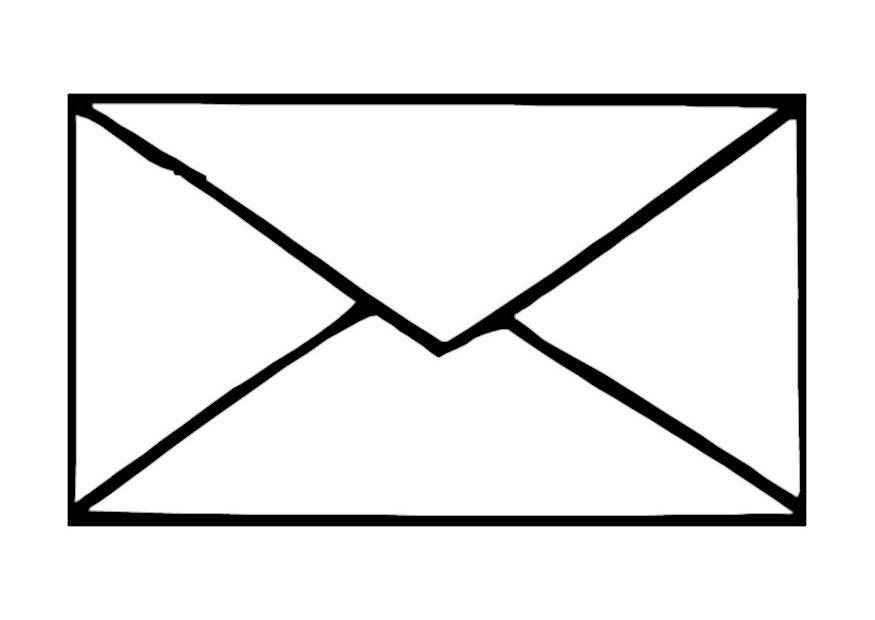
\includegraphics[width=4cm]{9Diff-LT.3-Abb_Umschlag.jpg}
	\end{wrapfigure}

	Eine Variable ist ein Platzhalter für einen Datenwert.

	Man kann sie sich wie einen Umschlag vorstellen, in den man eine Karte mit einer Zahl (oder einer anderen Information) steckt. Die Information kann jederzeit wieder hervorgeholt und benutzt werden. Es kann auch eine andere Karte mit einem neuen Wert in den Umschlag gesteckt werden.
	\end{wrapfix}

	\smallskip
	\begin{scratch}[scale=0.7]
		\blockvariable{setze \selectmenu{umschlag} auf \ovalnum{42}}
		\blocklook{sage \ovalvariable{umschlag}}
	\end{scratch}
	\smallskip

	Variablen in Scratch können \emph{lokal} oder \emph{global} sein.
	\begin{smallitem}
		\item \emph{Lokale Variablen} lernst Du im Zusammenhang mit \emph{Klonen} kennen (siehe \prettyref{hilfe:klone}).
		\item Jede \emph{globale Variablen} gibt es im ganzen Projekt genau einmal.
	\end{smallitem}

	Um eine neue Variable zu erstellen, wähle die Kategorie \enquote{Variablen} und klicke den Button \menu{Neue Variable}. Gib einen \emph{Namen} für die  neue Variable ein und Wähle \enquote{Für alle Figuren} für eine \emph{globale Variable} und \enquote{Nur für diese Figur} für eine \emph{lokale Variable}.
\end{hilfekarte}

\begin{loesungskarte}[Variablen]
	Die neue Variable taucht nun im Bereich \enquote{Variablen} auf und kann in den Skriptbereich gezogen werden. Hier findest Du auch weiter Blöcke, um mit Variablen zu arbeiten.

	\scratchinline{\blockvariable{setze \selectmenu{meine Variable} auf \ovalnum{0}}} ändert den Wert einer Variablen auf einen Neuen.

	\scratchinline{\blockvariable{ändere \selectmenu{meine Variable} um \ovalnum{0}}} addiert den angegebenen Wert auf den Wert, der aktuell in der Variablen gespeichert ist. Um zu subtrahieren gib eine negative Zahl an.

	\scratchinline{\blockvariable{zeige Variable \selectmenu{meine Variable}}} zeigt den Wert der Variablen oben links in der Bühne an. Die Werte können verschoben und durch Anklicken in der Größe verändert werden. (Zum Beispiel als Punktezähler.)

	\scratchinline{\blockvariable{verstecke Variable \selectmenu{meine Variable}}} zeigt eine Variable nicht mehr auf der Bühne an.
\end{loesungskarte}

\begin{hilfekarte}{Klone}{klone}
	\emph{Klone} sind Kopien einer Figur, die in einem Scratch-Programm erstellt werden können. Sie werden nicht in der Liste der Figuren angezeigt, sondern nur auf der Bühne. Eine Figur kann Skripte enthalten, die nur von \emph{Klonen} ausgeführt werden.

	Die Blöcke für Klone findest du unten im Bereich \enquote{Steuerung}.

	\scratchinline{\blockcontrol{erzeuge Klon von \ovalcontrol*{mir selbst}}} erzeugt einen Klon der Figur, in der der Block benutzt wird. Falls es mehrere Figuren gibt, kann auch ein Klon einer anderen Figur erzeugt werden.

	\scratchinline{\blockstop{lösche diesen Klon}} löscht den Klon, in dem der Block ausgeführt wird. Wenn der Block in der Originalfigur benutzt wird, passiert nichts.

	\scratchinline{\blockinitclone{Wenn ich als Klon entstehe}} startet ein Skript, das nur für Klone ausgeführt wird. Alle Blöcke unterhalb dieses Blocks werden ausgeführt, sobald ein Klon mit \scratchinline{\blockcontrol{erzeuge Klon von \ovalcontrol*{mir selbst}}} erzeugt wurde.
\end{hilfekarte}

\begin{loesungskarte}[Beispiel]
	Ergänze folgendes Skript in einer Ball-Figur.
	\begin{multicols}{2}
		\begin{scratch}
			\blockinit{Wenn \greenflag angeklickt wird}
			\blocklook{verstecke dich}
			\blockinfloop{wiederhole fortlaufend}{
				\blockcontrol{erzeuge Klon von \ovalcontrol*{mir selbst}}
			}
		\end{scratch}

		\columnbreak

		\begin{scratch}
			\blockinitclone{Wenn ich als Klon entstehe}
			\blockmove{gehe zu \ovalmove*{Zufallsposition}}
			\blocklook{wechsle zu Kostüm  \ovaloperator{Zufallszahl \ovalnum{1} bis \ovalnum{5}}}
			\blocklook{zeige dich}
			\blockrepeat{wiederhole \ovalnum{20} mal}{
				\blocklook{ändere Effekt \selectmenu{Durchsichtigkeit} um \ovalnum{5}}
			}
			\blockstop{lösche diesen Klon}
		\end{scratch}
	\end{multicols}
\end{loesungskarte}

\begin{hilfekarte}{Nachrichten}{nachrichten}
	\emph{Nachrichten} sind Signale, die zwischen Figuren verschickt werden können. Eine Figur sendet ein Signal und die anderen Figuren können darauf reagieren.

	Eine neue Nachricht kann erstellt werden, indem in einem der Nachrichten-Blöcke unten auf den kleinen Pfeil geklickt wird und \enquote{Neue Nachricht} ausgewählt wird.

	Die Blöcke für Nachrichten findest du unten im Bereich \enquote{Ereignisse}.

	\scratchinline{\blockevent{sende \ovalcontrol*{Nachricht} an alle}} sendet eine Nachricht an alle anderen Figuren.

	\scratchinline{\blockevent{sende \ovalcontrol*{Nachricht} an alle und warte}} sendet eine Nachricht an alle anderen Figuren und wartet darauf, dass alle Skripte, die auf diese Nachricht reagieren, gestoppt haben.

	\scratchinline{\blockinit{Wenn ich \selectmenu{Nachricht} empfange}} startet ein Skript, nachdem eine Nachricht empfangen wurde. Alle Blöcke unterhalb dieses Blocks werden ausgeführt, sobald die Nachricht mit \scratchinline{\blockevent{sende \ovalcontrol*{Nachricht} an alle}} gesendet wurde.
\end{hilfekarte}

\begin{loesungskarte}[Beispiel]
	Erstelle einige Überraschungsfiguren und ergänze in jeder folgendes Skript:

	\begin{scratch}
		\blockinit{Wenn ich \selectmenu{farbe} empfange}
		\blocklook{setze Effekt \selectmenu{Farbe} auf \ovaloperator{Zuffalszahl \ovalnum{0} bis \ovalnum{200}}}
	\end{scratch}
	\bigskip

	Ergänze dieses Skript in der Bühne:

	\begin{scratch}
		\blockinit{Wenn Taste \selectmenu{Leertaste} gedrückt wird}
		\blockevent{sende \ovalcontrol*{farbe} an alle}
	\end{scratch}
\end{loesungskarte}



\begin{karte1}{Variablen}
	\hilfeMarke{variablen}
	Mit Variablen lassen sich Informationen in einem Skript speichern und wieder abrufen.

	\begin{center}
		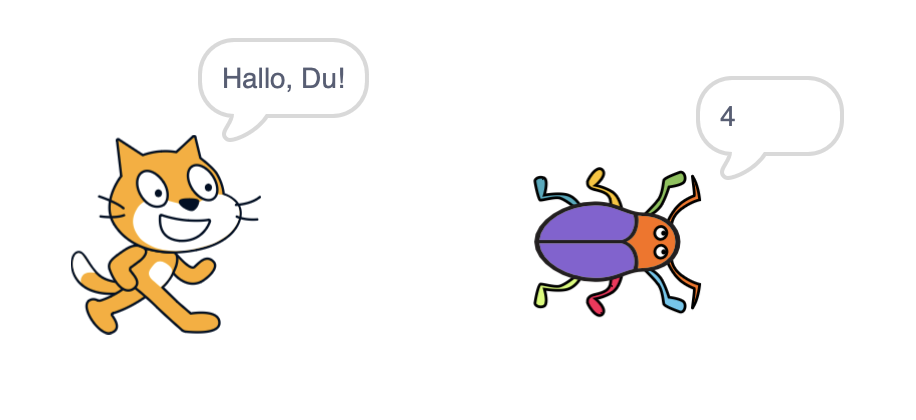
\includegraphics[width=8cm]{9Diff-LT.3-Abb_Variablen.png}
	\end{center}

	\textbf{Aufgabe:} Erstelle zwei Figuren.

	Erstelle zwei Variablen \emph{für alle Figuren}: \enquote{zahl} und \enquote{text}. Wenn die eine Figur angeklickt wird, wird \enquote{zahl} um \code{1} geändert. Wenn die andere Figur angeklickt wird, fragt sie nach einer Texteingabe und setzt \enquote{text} auf die Antwort.

	Beim Betätigen der Leertaste \enquote{sagen} beide Figuren die jeweils die Variable, die sie verändert haben.
\end{karte1}

\begin{loesungskarte}
	\begin{multicols}{2}
		In Figur 1:

		\begin{scratch}[scale=0.7]
			\blockinit{Wenn diese Figur angeklickt wird}
			\blockvariable{ändere \selectmenu{zahl} um \ovalnum{1}}
		\end{scratch}

		\begin{scratch}[scale=0.7]
			\blockinit{Wenn Taste \selectmenu{Leertaste} gedrückt wird}
			\blocklook{sage \ovalvariable{zawhl} für \ovalnum{2} Sekunden}
		\end{scratch}
		\columnbreak

		In Figur 2:

		\begin{scratch}[scale=0.7]
			\blockinit{Wenn diese Figur angeklickt wird}
			\blocksensing{frage \ovalnum{Gib etwas ein.} und warte}
			\blockvariable{setze \selectmenu{text} auf \ovalsensing{Antwort}}
		\end{scratch}

		\begin{scratch}[scale=0.7]
			\blockinit{Wenn Taste \selectmenu{Leertaste} gedrückt wird}
			\blocklook{sage \ovalvariable{text} für \ovalnum{2} Sekunden}
		\end{scratch}
	\end{multicols}
\end{loesungskarte}

\begin{karte2}{Figuren klonen}
	\hilfeMarke{klone}
Jede Figur in Scratch kann \emph{geklont} werden. Das bedeutet, eine Kopie der Figur wird auf der Bühne erstellt.

Sobald ein Klon entsteht, führt er die Anweisungen aus, die unterhalb von \begin{inlinescratch}\blockinitclone{Wenn ich als Klon entstehe}\end{inlinescratch} stehen. So kann mit nur einer Figur die gesamte Bühne gefüllt werden. Ein Klon kann mit \begin{inlinescratch}\blockstop{lösche diesen Klon}\end{inlinescratch} wieder von der Bühne entfernt werden.

\textbf{Aufgabe:} Erstelle in einem Scratch-Programm eine Ballon-Figur mit folgendem Programm:

\begin{scratch}[scale=0.7]
	\blockinit{Wenn \greenflag angeklickt wird}
	\blocklook{verstecke dich}
	\blockinfloop{wiederhole fortlaufend}{
		\blockcontrol{erzeuge Klon von \ovalcontrol*{mir selbst}}
		\blockcontrol{warte \ovaloperator{Zufallszahl von \ovalnum{0.2} bis \ovalnum{0.8}} Sekunden}
	}
\end{scratch}
\smallskip

Ergänze das Programm so, dass die Klone des Ballons an eine zufällige Position am unteren Bühnenrand bewegt und angezeigt werden. Die Klone sollen dann langsam nach oben steigen, bis sie die Bühne verlassen. Dann werden sie gelöscht.
\end{karte2}

\begin{loesungskarte}
\begin{center}
	\begin{scratch}
		\blockinitclone{Wenn ich als Klon entstehe}
		\blocklook{setze Effekt \selectmenu{Farbe} auf \ovaloperator{Zufallszahl \ovalnum{1} bis \ovalnum{255}}}
		\blockmove{gehe zu x: \ovaloperator{Zufallszahl von \ovalnum{-200} bis \ovalnum{200} y: \ovalnum{-250}}}
		\blocklook{zeige dich}
		\blockrepeat{wiederhole bis \booloperator{\ovalmove{y-Position} > \ovalnum{210}}}{
			\blockmove{ändere y um \ovalnum{10}}
			\blockmove{ändere x um \ovaloperator{\selectmenu{sin} von \ovalmove{y-Position}}}
		}
		\blockstop{lösche diesen Klon}
	\end{scratch}
\end{center}

Der Befehl \begin{inlinescratch}\blockmove{ändere x um \ovaloperator{\selectmenu{sin} von \ovalmove{y-Position}}}\end{inlinescratch} sorgt dafür, dass die Ballons \enquote{hin und her} schweben. \begin{inlinescratch}\blocklook{setze Effekt \selectmenu{Farbe} auf \ovaloperator{Zufallszahl \ovalnum{1} bis \ovalnum{255}}}\end{inlinescratch} ändert die Farbe der Klone.
\end{loesungskarte}

\begin{karte2}{Lokale Variablen}
	\hilfeMarke{klone}\small
	In Scratch gibt es zwei Arten von Variablen: \emph{lokale} und \emph{globale}.

	\emph{Lokale Variablen} werden für eine Figur erstellt und enthalten einen eigenen Wert \emph{für jeden Klon der Figur}, der mit \begin{inlinescratch}\blockinitclone{Wenn ich als Klon entstehe}\end{inlinescratch} erstellt wird. Wähle dazu \enquote{Nur für diese Figur} beim Erstellen der Variablen aus.

	\bigskip
	\textbf{Aufgabe:} Erstelle eine Rocketship-Figur mit einer lokalen Variable \enquote{speed} und folgendem Programm:

	\begin{scratch}[scale=0.7]
		\blockinit{Wenn \greenflag angeklickt wird}
		\blocklook{verstecke dich}
		\blockinfloop{wiederhole fortlaufend}{
			\blockcontrol{erzeuge Klon von \ovalcontrol*{mir selbst}}
			\blockcontrol{warte \ovalnum{.2} Sekunden}
		}
	\end{scratch}
	\smallskip

	Ergänze dann das Programm so, dass die Klone der Rakete immer schneller abheben, indem sich ihre y-Koordinate immer um \enquote{speed} ändert und \enquote{speed} immer um \code{1} erhöht wird. Am oberen Rand der Bühne wird der Klon gelöscht.

	\textbf{Tipp:} Setze die Variable \enquote{speed} zuerst auf \code{1} und nutze eine \enquote{wiederhole bis} Schleife.
\end{karte2}

\begin{loesungskarte}
	\begin{center}
		\begin{scratch}
			\blockinitclone{Wenn ich als Klon entstehe}
			\blockvariable{setze \selectmenu{speed} auf \ovalnum{1}}
			\blockmove{gehe zu x: \ovaloperator{Zufallszahl von \ovalnum{-200} bis \ovalnum{200} y: \ovalnum{-172}}}
			\blocklook{zeige dich}
			\blockrepeat{wiederhole bis \booloperator{\ovalmove{y-Position} > \ovalnum{210}}}{
				\blockmove{ändere y um \ovalvariable{speed}}
				\blockvariable{ändere \selectmenu{speed} um \ovalnum{2}}
			}
			\blockstop{lösche diesen Klon}
		\end{scratch}
	\end{center}
\end{loesungskarte}

\begin{karte2}{Nachrichten}
	\hilfeMarke{nachrichten}
	\emph{Nachrichten} werden von einer Figur an alle anderen gesendet. Die Empfänger können dann auf diese Signale reagieren. Eine Nachricht enthält keine Informationen (zum Beispiel einen Zahlwert), sondern nur das Signal selbst.

	Die Blöcke für Nachrichten findest Du unten im Bereich \enquote{Ereignisse}.

	\bigskip
	\textbf{Aufgabe:} Erstelle mehrere Figuren von tanzenden Menschen und jede mit dem folgenden Programm:

	\begin{scratch}[scale=0.7]
		\blockinfloop{wiederhole fortlaufend}{
			\blocklook{wechsle zum nächsten Kostüm}
			\blockcontrol{warte \ovalnum{.5} Sekunden}
		}
	\end{scratch}
	\smallskip

	Ergänze die Programme so, dass die Wiederholung ausgelöst wird, wenn die Nachricht \code{tanzen} empfangen wird. Ergänze in der Bühne ein Skript, dass beim Betätigen der Leertaste die Nachricht \code{tanzen} an alle Figuren sendet.

	Programmiere dann eine \code{stopp} Nachricht, die bei einer anderen Taste gesendet wird und die Tänzer stoppen lässt.
\end{karte2}

\begin{loesungskarte}
\begin{multicols}{2}
	In jeder Figur:

	\begin{scratch}[scale=0.7]
		\blockinit{Wenn ich \selectmenu{tanzen} empfange}
		\blockinfloop{wiederhole fortlaufend}{
			\blocklook{wechsle zum nächsten Kostüm}
			\blockcontrol{warte \ovalnum{.5} Sekunden}
		}
	\end{scratch}

	\begin{scratch}[scale=0.7]
		\blockinit{Wenn ich \selectmenu{stopp} empfange}
		\blockcontrol{stoppe \selectmenu{andere Skripte der Figur}}
	\end{scratch}
	\columnbreak

	In der Bühne:

	\begin{scratch}[scale=0.7]
		\blockinit{Wenn Taste \selectmenu{Leertaste} gedrückt wird}
		\blockevent{sende \ovalcontrol*{tanzen} an alle}
	\end{scratch}

	\begin{scratch}[scale=0.7]
		\blockinit{Wenn Taste \selectmenu{s} gedrückt wird}
		\blockevent{sende \ovalcontrol*{stopp} an alle}
	\end{scratch}
\end{multicols}
\end{loesungskarte}


\begin{karte3}{Listen}
	\hilfeMarke{variablen}
	\emph{Listen} sind spezielle \emph{Variablen}, die nicht nur einen Wert, sondern eine ganze Reihe von individuellen Werten speichern können.

	Wähle im Bereich \enquote{Variablen} den Button \menu{Neue Liste}, um eine Liste zu erstellen. Unterhalb des Buttons werde nun neue Blöcke angezeigt, mit denen Werte in der Liste gespeichert und aus dieser hervorgeholt werden können.

	\textbf{Aufgabe:} Erstelle ein Programm, das in einer Liste \enquote{tonhöhen} zehn Zufallszahlen zwischen 1 und 100 speichert.

	Danach wird die Tonhöhe auf den ersten Wert der Liste eingestellt, der Klang \enquote{Pop} abgespielt und das erste Element aus der Liste gelöscht. Dies passiert so lange, bis die Liste leer ist (Länge der Liste gleich Null).

	\textbf{Offene Aufgabe:} Modifiziere das Programm auf kreative Weise. Kannst Du zum Beispiel ein Lied spielen lassen?
\end{karte3}

\begin{loesungskarte}
	\begin{center}
		\begin{scratch}
			\blockinit{Wenn \greenflag angeklickt wird}
			\blocklist{lösche alles aus \selectmenu{tonhöhen}}
			\blockrepeat{wiederhole \ovalnum{10} mal}{
				\blocklist{füge \ovaloperator{Zufallszahl von \ovalnum{1} bis \ovalnum{100}} zu \selectmenu{tonhöhe} hinzu}
			}
			\blockrepeat{wiederhole bis \booloperator{\ovallist{Länge von \selectmenu{tonhöhe}} = \ovalnum{0}}}{
				\blocksound{setze Effekt \selectmenu{Höhe} auf \ovallist{Element \ovalnum{1} von \selectmenu{tonhöhe}}}
				\blocklist{lösche \ovalnum{1} aus \selectmenu{tonhöhe}}
				\blocksound{spiele Klang \ovalsound*{pop} ganz}
			}
		\end{scratch}
	\end{center}
\end{loesungskarte}

\end{document}
